\documentclass{beamer}

\usepackage[utf8]{inputenc}
\usepackage[T1]{fontenc}
\usepackage{graphicx}
\usepackage{amsmath}
\usepackage{hyperref}
\usepackage{xcolor}

\usepackage{booktabs}
\usepackage{tikz}
\usepackage{babel}
\usetikzlibrary{shapes.geometric}
\usetikzlibrary{positioning}

\usepackage{todonotes}
\usepackage{listings}

\usepackage{subcaption}
\usepackage{algorithm}
\usepackage{algorithmic}
\usepackage{amsmath}
\usepackage{amssymb}
\usepackage{amsfonts}
\usepackage{dsfont}
\usepackage{xspace}
\usepackage{xr}
\usepackage{multirow}
\usepackage{multicol}
\usepackage{siunitx}
\usepackage{afterpage}

\usepackage{enumerate}
\usepackage{soul}
\usepackage{mathtools}

\usetheme{metropolis} 
\usecolortheme{beaver} 


\title{PolScience: Research4Revenue's candidates identification database.}
\author{Cyprien Fourcroy, Wojtek Kutak, Suren Mnatsakanyan,  Marek Mytkowski, Michał Puścian \\
\textbf{Supervisor:} Elżbieta Sienkiewicz, \textbf{Project initiator:} Robert Sitnik} 


\begin{document}

\frame{\titlepage}

\begin{frame}{Introduction}
    \framesubtitle{The Problem: Finding Scientists is Hard}
    \begin{itemize}
        \item Academic research has big potential for commercial business.
        \item Connecting universities with industry remains a major bottleneck.
        \item \textbf{Research4Revenue:} A project to find and train active Polish scientists in industry collaboration.
        \item \textbf{The Old Way:} Manual searches across messy university websites.
        \item \textbf{The Solution:} Automate the discovery process.
    \end{itemize}
\end{frame}

\begin{frame}{Introduction}
    \framesubtitle{Project Goals: Our Target}
    \begin{itemize}
        \item Build a central database of Polish scientists with a search tool.
        \item \textbf{Data Collection:} Automatically scrape names, papers, and projects.
        \item \textbf{Filtering:} Filter candidates by degrees, publication counts, or industry collaboration projects.
        \item \textbf{Semantic search:} Match natural language query to profile keywords and publication titles.
        \item \textbf{The Strategy:} Run a heavy pipeline once a year to capture a data snapshot.
        \item Use NLP and database queries to easily pick the final scientist cohort.
    \end{itemize}
\end{frame}

\begin{frame}{Data Collection}
    \framesubtitle{The Source and The Pipeline}
    \begin{itemize}
        \item \textbf{Our Target:} The official \textit{Ludzie Nauki} (People of Science) portal.
        \item Huge dataset: Over 200k scientists, 2M publications, plus patents.
        \item We built a custom data pipeline to download everything into local SQLite.
        \item We used the public JSON API with strict rate limits to avoid server bans.
        \item The process requires 4 separate passes due to complex API endpoints.
    \end{itemize}
\end{frame}

\begin{frame}[fragile]{Data Collection}
    \framesubtitle{The 4-Pass Pipeline Architecture}
    \centering
    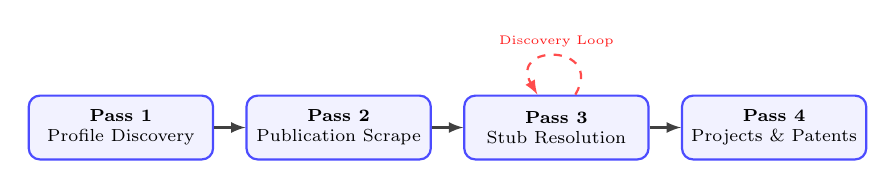
\begin{tikzpicture}[
        node distance=0.8cm and 0.4cm,
        box/.style={rectangle, draw=blue!70, fill=blue!5, thick, rounded corners, minimum width=2.6cm, minimum height=0.9cm, align=center, font=\scriptsize},
        arrow/.style={-latex, thick, color=darkgray},
        looparrow/.style={-latex, thick, color=red!70, dashed},
        scale=0.9, every node/.style={scale=0.9}
    ]

        
        \node[box] (pass1) {\textbf{Pass 1} \\ Profile Discovery};
        \node[box, right=of {pass1}] (pass2) {\textbf{Pass 2} \\ Publication Scrape};
        \node[box, right=of {pass2}] (pass3) {\textbf{Pass 3} \\ Stub Resolution};
        \node[box, right=of {pass3}] (pass4) {\textbf{Pass 4} \\ Projects \& Patents};
        
        
        \draw[arrow] (pass1) -- (pass2);
        \draw[arrow] (pass2) -- (pass3);
        \draw[arrow] (pass3) -- (pass4);
        
        
        \path (pass3) edge [looparrow, out=60, in=120, looseness=4] node[above, font=\tiny, color=red!90] {Discovery Loop} (pass3);
    \end{tikzpicture}
    
    \vspace{0.3cm}
    \begin{itemize}
        \item \textbf{Pass 1 \& 2:} Discover scientists' profiles and scrape their articles, flagging missing co-authors as "stubs".
        \item \textbf{Pass 3 Loop:} Recursively fetch profile details for "stubs" until there are only complete profile.
        \item \textbf{Pass 4:} For each profile scrape projects and patents.
    \end{itemize}
\end{frame}

\begin{frame}{Data Collection}
    \framesubtitle{Pass 1 \& 2: Breaking the Limits and Finding Clues}
    \begin{itemize}
        \item \textbf{Pass 1 --- Profile Discovery:}
        \begin{itemize}
            \item The API limits results to 1000 items per search query.
            \item \textbf{Our Trick:} Split searches by discipline and sort text A-Z and Z-A.
            \item Doubled our limit to 2000 profiles per mix; captured 68,147 profiles.
        \end{itemize}
        \item \textbf{Pass 2 --- Gathering Publications:}
        \begin{itemize}
            \item Downloaded scientific papers' metadata and saved authorship connections.
            \item Extract keywords if present in Ludzie Nauka.
            \item Found hidden co-authors and created temporary "stub" profiles.
        \end{itemize}
    \end{itemize}
\end{frame}

\begin{frame}{Data Collection}
    \framesubtitle{Pass 3 \& 4: Filling the Gaps}
    \begin{itemize}
        \item \textbf{Pass 3 --- Resolving the Stubs:}
        \begin{itemize}
            \item An iterative loop to investigate the hidden co-authors.
            \item Downloaded full profiles and papers for every temporary stub.
            \item Loop stopped when stubs were cleared, yielding 165k rich profiles.
        \end{itemize}
        \item \textbf{Pass 4 --- Projects and Patents:}
        \begin{itemize}
            \item Scrape projects and patents related to every scientist's profile in our database.
            \item Gathered about 90k research projects and 17k patents.
        \end{itemize}
    \end{itemize}
\end{frame}

\begin{frame}{Data Collection}
    \framesubtitle{The Snapshot in Numbers}
    \begin{itemize}
        \item We successfully downloaded roughly $\frac{3}{4}$ of the entire platform.
    \end{itemize}
    \begin{table}
        \centering
        \small
        \begin{tabular}{lr}
            \hline
            \textbf{Collected Entity} & \textbf{Total Count} \\
            \hline
            Scientist Profiles & 165,346 \\
            Publications & 1,510,279 \\
            Research Projects & 90,493 \\
            Patents \& Property Rights & 33,576 \\
            \hline
        \end{tabular}
    \end{table}
\end{frame}

\begin{frame}{Data Collection}
    \framesubtitle{Data Quality and Collaboration Insights}
    \begin{itemize}
        \item \textbf{The ID Gap:} About 50\% of scientists lack ORCID, and 48\% of papers lack DOI.
        \item \textbf{Team Sizes:} Patents usually have the largest teams, while projects have the smallest.
    \end{itemize}
    
    \begin{table}
        \centering
        \footnotesize
        \begin{tabular}{lrr}
            \hline
            \textbf{Target ID} & \textbf{Has ID Value} & \textbf{Missing ID Value} \\
            \hline
            Profile ORCID & 49.1\% & 50.9\% \\
            Publication DOI & 52.0\% & 48.0\% \\
            \hline
        \end{tabular}
    \end{table}

    \begin{table}
        \centering
        \footnotesize
        \begin{tabular}{lr}
            \hline
            \textbf{Entity Type} & \textbf{Average Authors per Item} \\
            \hline
            Publication & 2.27 \\
            Research Project & 1.76 \\
            Patent / Patent Right & 2.50 / 2.67 \\
            \hline
        \end{tabular}
    \end{table}
\end{frame}

\begin{frame}{Expert search application}
    \framesubtitle{From topic query to ranked candidates}
    \begin{itemize}
        \item Natural-language \textbf{topic query} $\rightarrow$ ranked list of scientists for Research4Revenue outreach.
        \item Satisfies \textbf{Candidate Filtering}: topic match plus structural rules (publications, projects, degree, institution).
        \item \textbf{Two phases:}
        \begin{itemize}
            \item \textbf{Offline} --- \texttt{build-index} rebuilds search artifacts after each DB snapshot.
            \item \textbf{Online} --- FastAPI web UI or CLI fuses three signals into a final ranking.
        \end{itemize}
        \item Indexed scope: \num{165346} non-stub profiles from our Ludzie Nauki snapshot.
    \end{itemize}
\end{frame}

\begin{frame}{Expert search pipeline}
    \framesubtitle{Offline build and query-time retrieval}
    \small
    \textbf{Build-index} (per search mode, shared co-auth graph):
    \begin{enumerate}
        \item Searchable text document per scientist
        \item BM25 index + multilingual embedding matrix
        \item Co-authorship graph over all indexed profiles
        \item Precomputed \textbf{co-auth degree} and \textbf{global PageRank}
    \end{enumerate}
    \vspace{0.25cm}
    \textbf{Query time} (over BM25 pool of top \num{5000}):
    \begin{enumerate}
        \item \textbf{Keywords} (BM25) \hfill
        \item \textbf{Structural filters} (optional)
        \item \textbf{Semantic} (cosine, MiniLM-L12-v2)
        \item \textbf{Community} (PPR, $\alpha=0.85$, seeds from top \num{200} BM25 hits)
    \end{enumerate}
    \vspace{0.2cm}
    \textbf{Two modes:} \textit{Publications} (titles + keywords) vs.\ \textit{Profile} (domains, specialties, institutions --- no titles).
\end{frame}

\begin{frame}{Score fusion}
    \framesubtitle{Normalise each signal, then combine}
    \begin{itemize}
        \item Each raw score min--max normalised \emph{over the current candidate pool} (missing $\rightarrow$ 0).
        \item User weights $w_{\mathrm{b}}, w_{\mathrm{e}}, w_{\mathrm{r}}$ renormalised to sum to 1.
    \end{itemize}
    \[
        \mathrm{Final}(p) = w'_{\mathrm{b}}\,\widehat{b}(p) + w'_{\mathrm{e}}\,\widehat{e}(p) + w'_{\mathrm{r}}\,\widehat{r}(p)
    \]
    \small
    $\widehat{b}$ = Keywords (BM25), $\widehat{e}$ = Semantic, $\widehat{r}$ = Community (PPR).
    \vspace{0.3cm}

    \begin{table}
        \centering
        \footnotesize
        \begin{tabular}{lr}
            \toprule
            \textbf{Parameter} & \textbf{Default} \\
            \midrule
            Recall pool & \num{5000} \\
            Results returned & \num{1000} \\
            Weights (Keywords / Semantic / Community) & 0.25 / 0.55 / 0.20 \\
            PPR restart $\alpha$ & 0.85 \\
            \bottomrule
        \end{tabular}
    \end{table}
\end{frame}

\begin{frame}{Network statistics}
    \framesubtitle{National co-authorship context per result}
    \begin{itemize}
        \item Graph: \num{165346} nodes; edge if $\geq$1 shared publication (weight = count).
        \item \textbf{Co-auth degree} --- number of distinct co-authors in the search graph.
        \item \textbf{Network rank} --- global PageRank on that graph (query-independent).
        \item \textbf{Cluster} --- modularity community hub label (optional GEXF export).
        \item Display columns are for human review; they do \textbf{not} change \textbf{Final} when query PPR is on.
        \item \textbf{Community} column = query-specific PPR score used in fusion (hidden if PPR disabled).
    \end{itemize}
\end{frame}

\begin{frame}{Web interface and validation}
    \framesubtitle{Browser UI, CSV export, automated tests}
    \begin{columns}[T,onlytextwidth]
        \column{0.52\textwidth}
        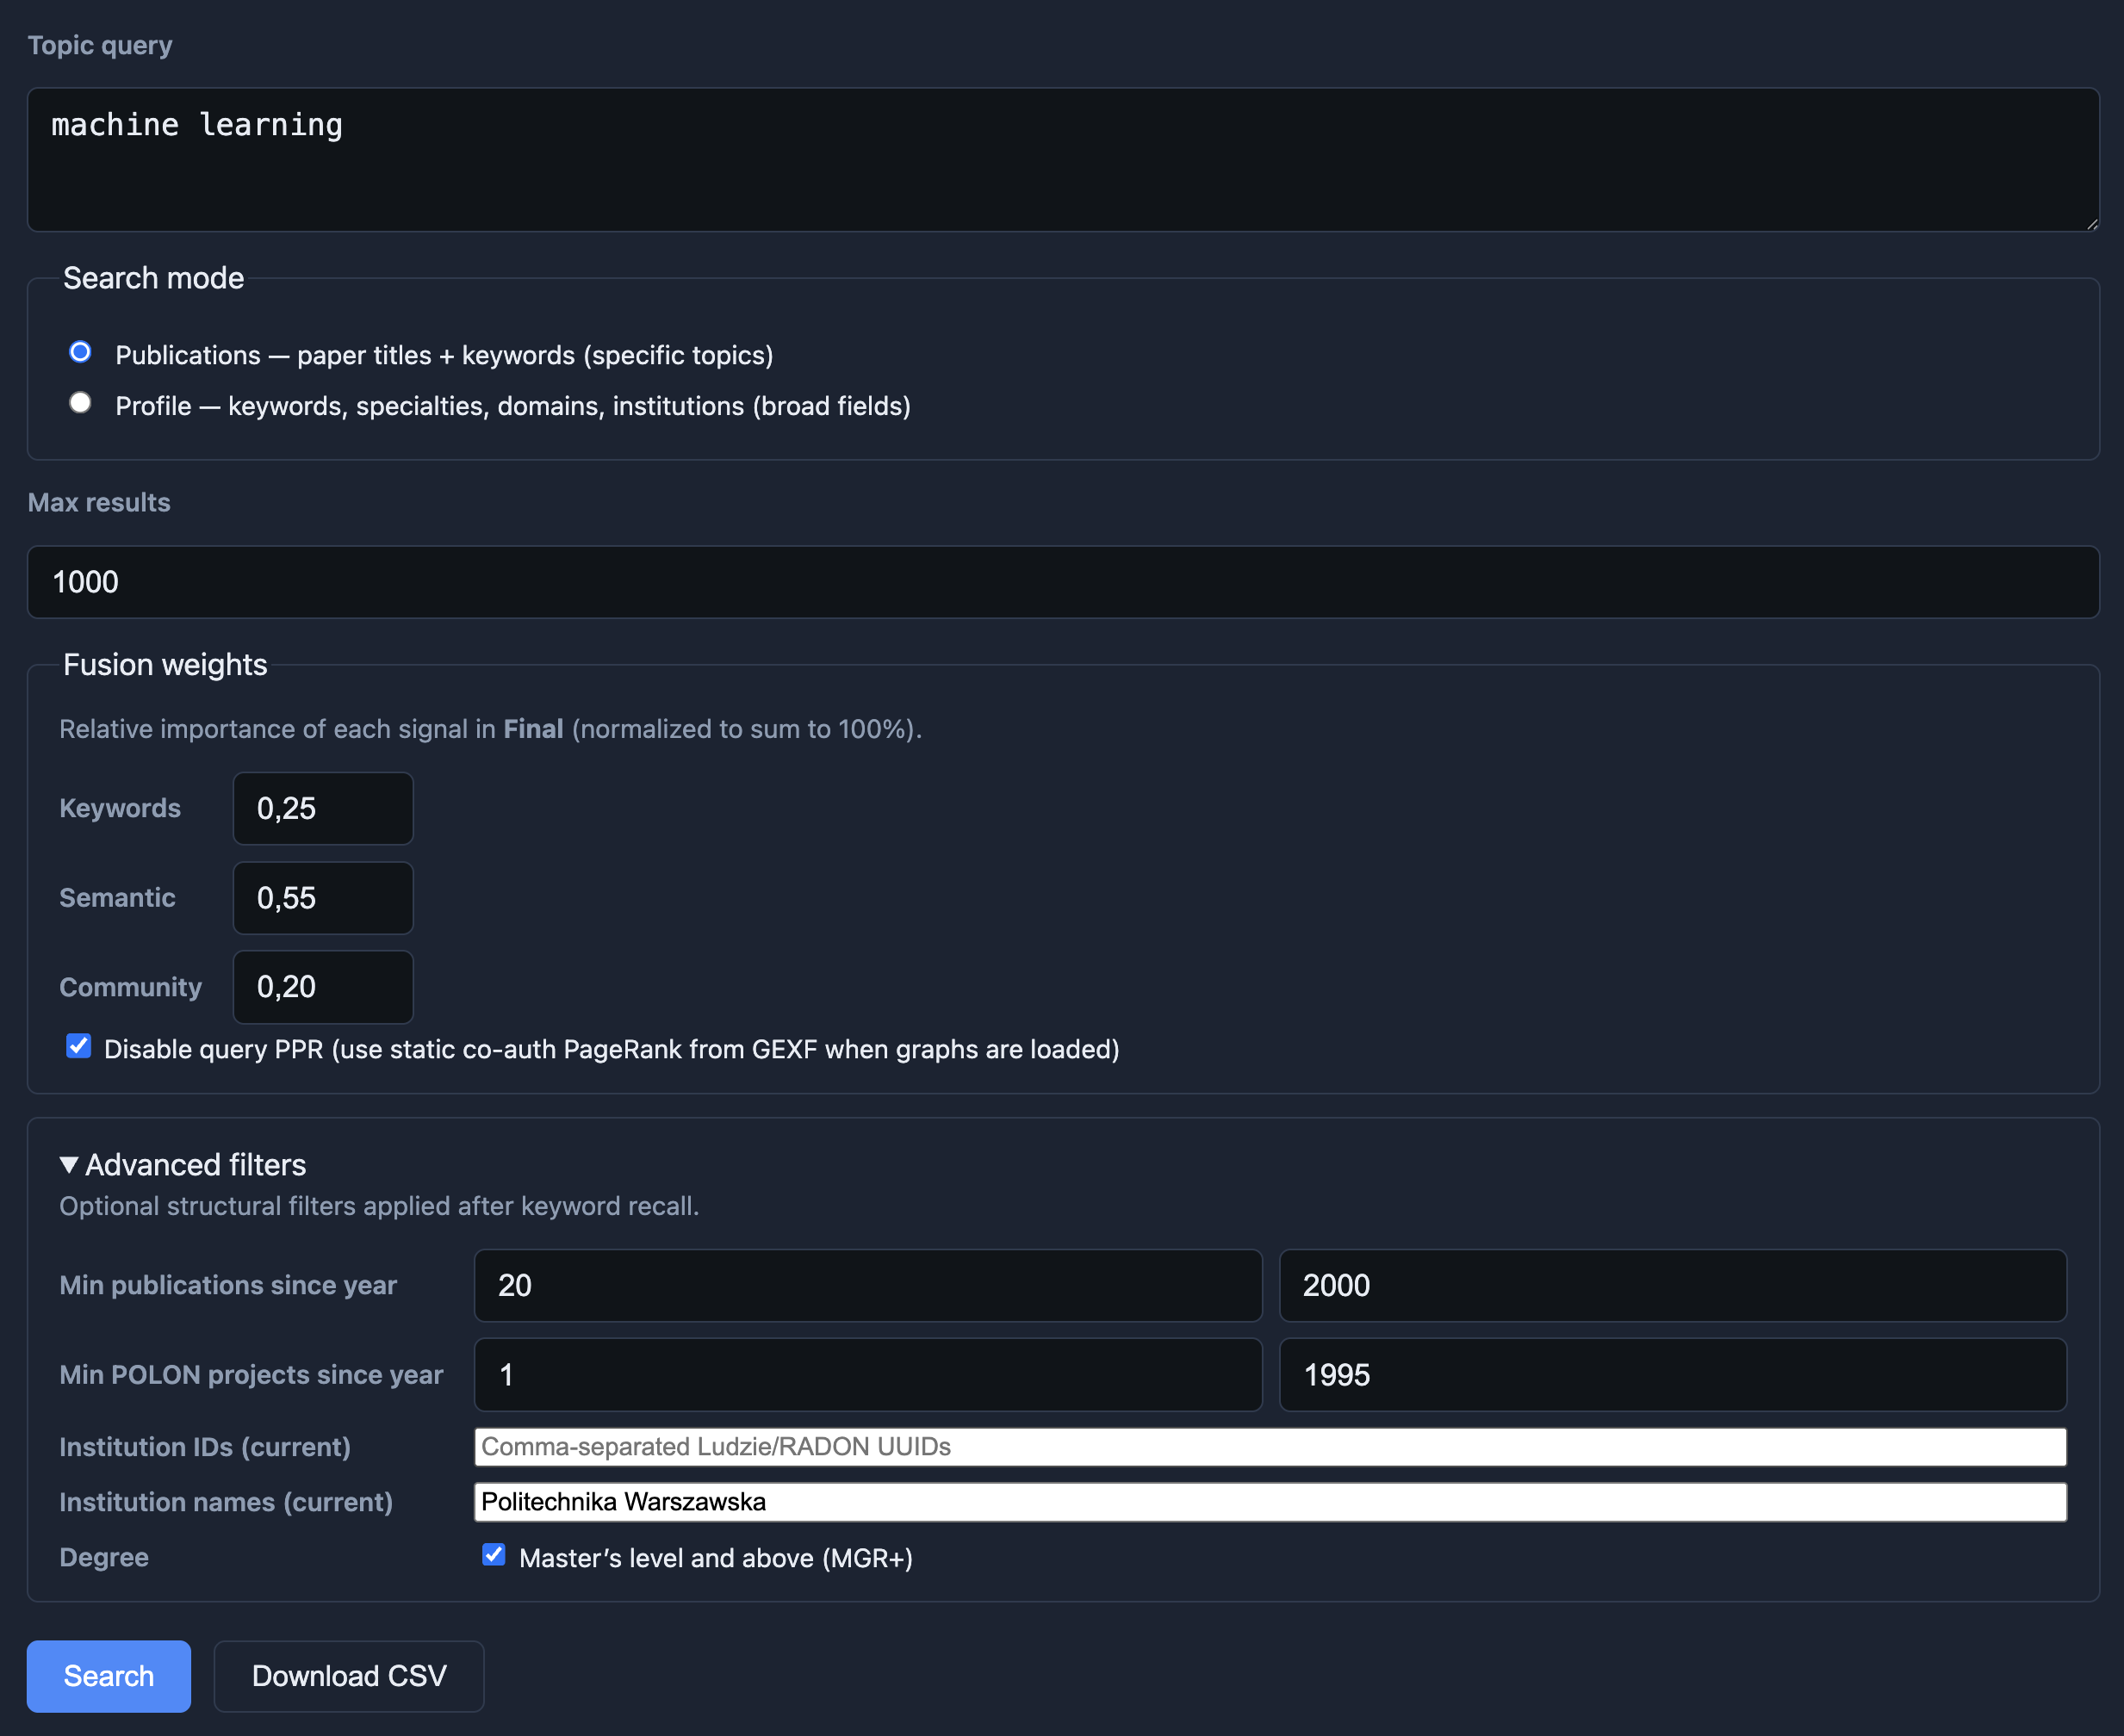
\includegraphics[width=\linewidth]{app_menu.png}
        \vspace{0.15cm}
        {\scriptsize Search form: query, mode, fusion weights, advanced filters.}
        \column{0.46\textwidth}
        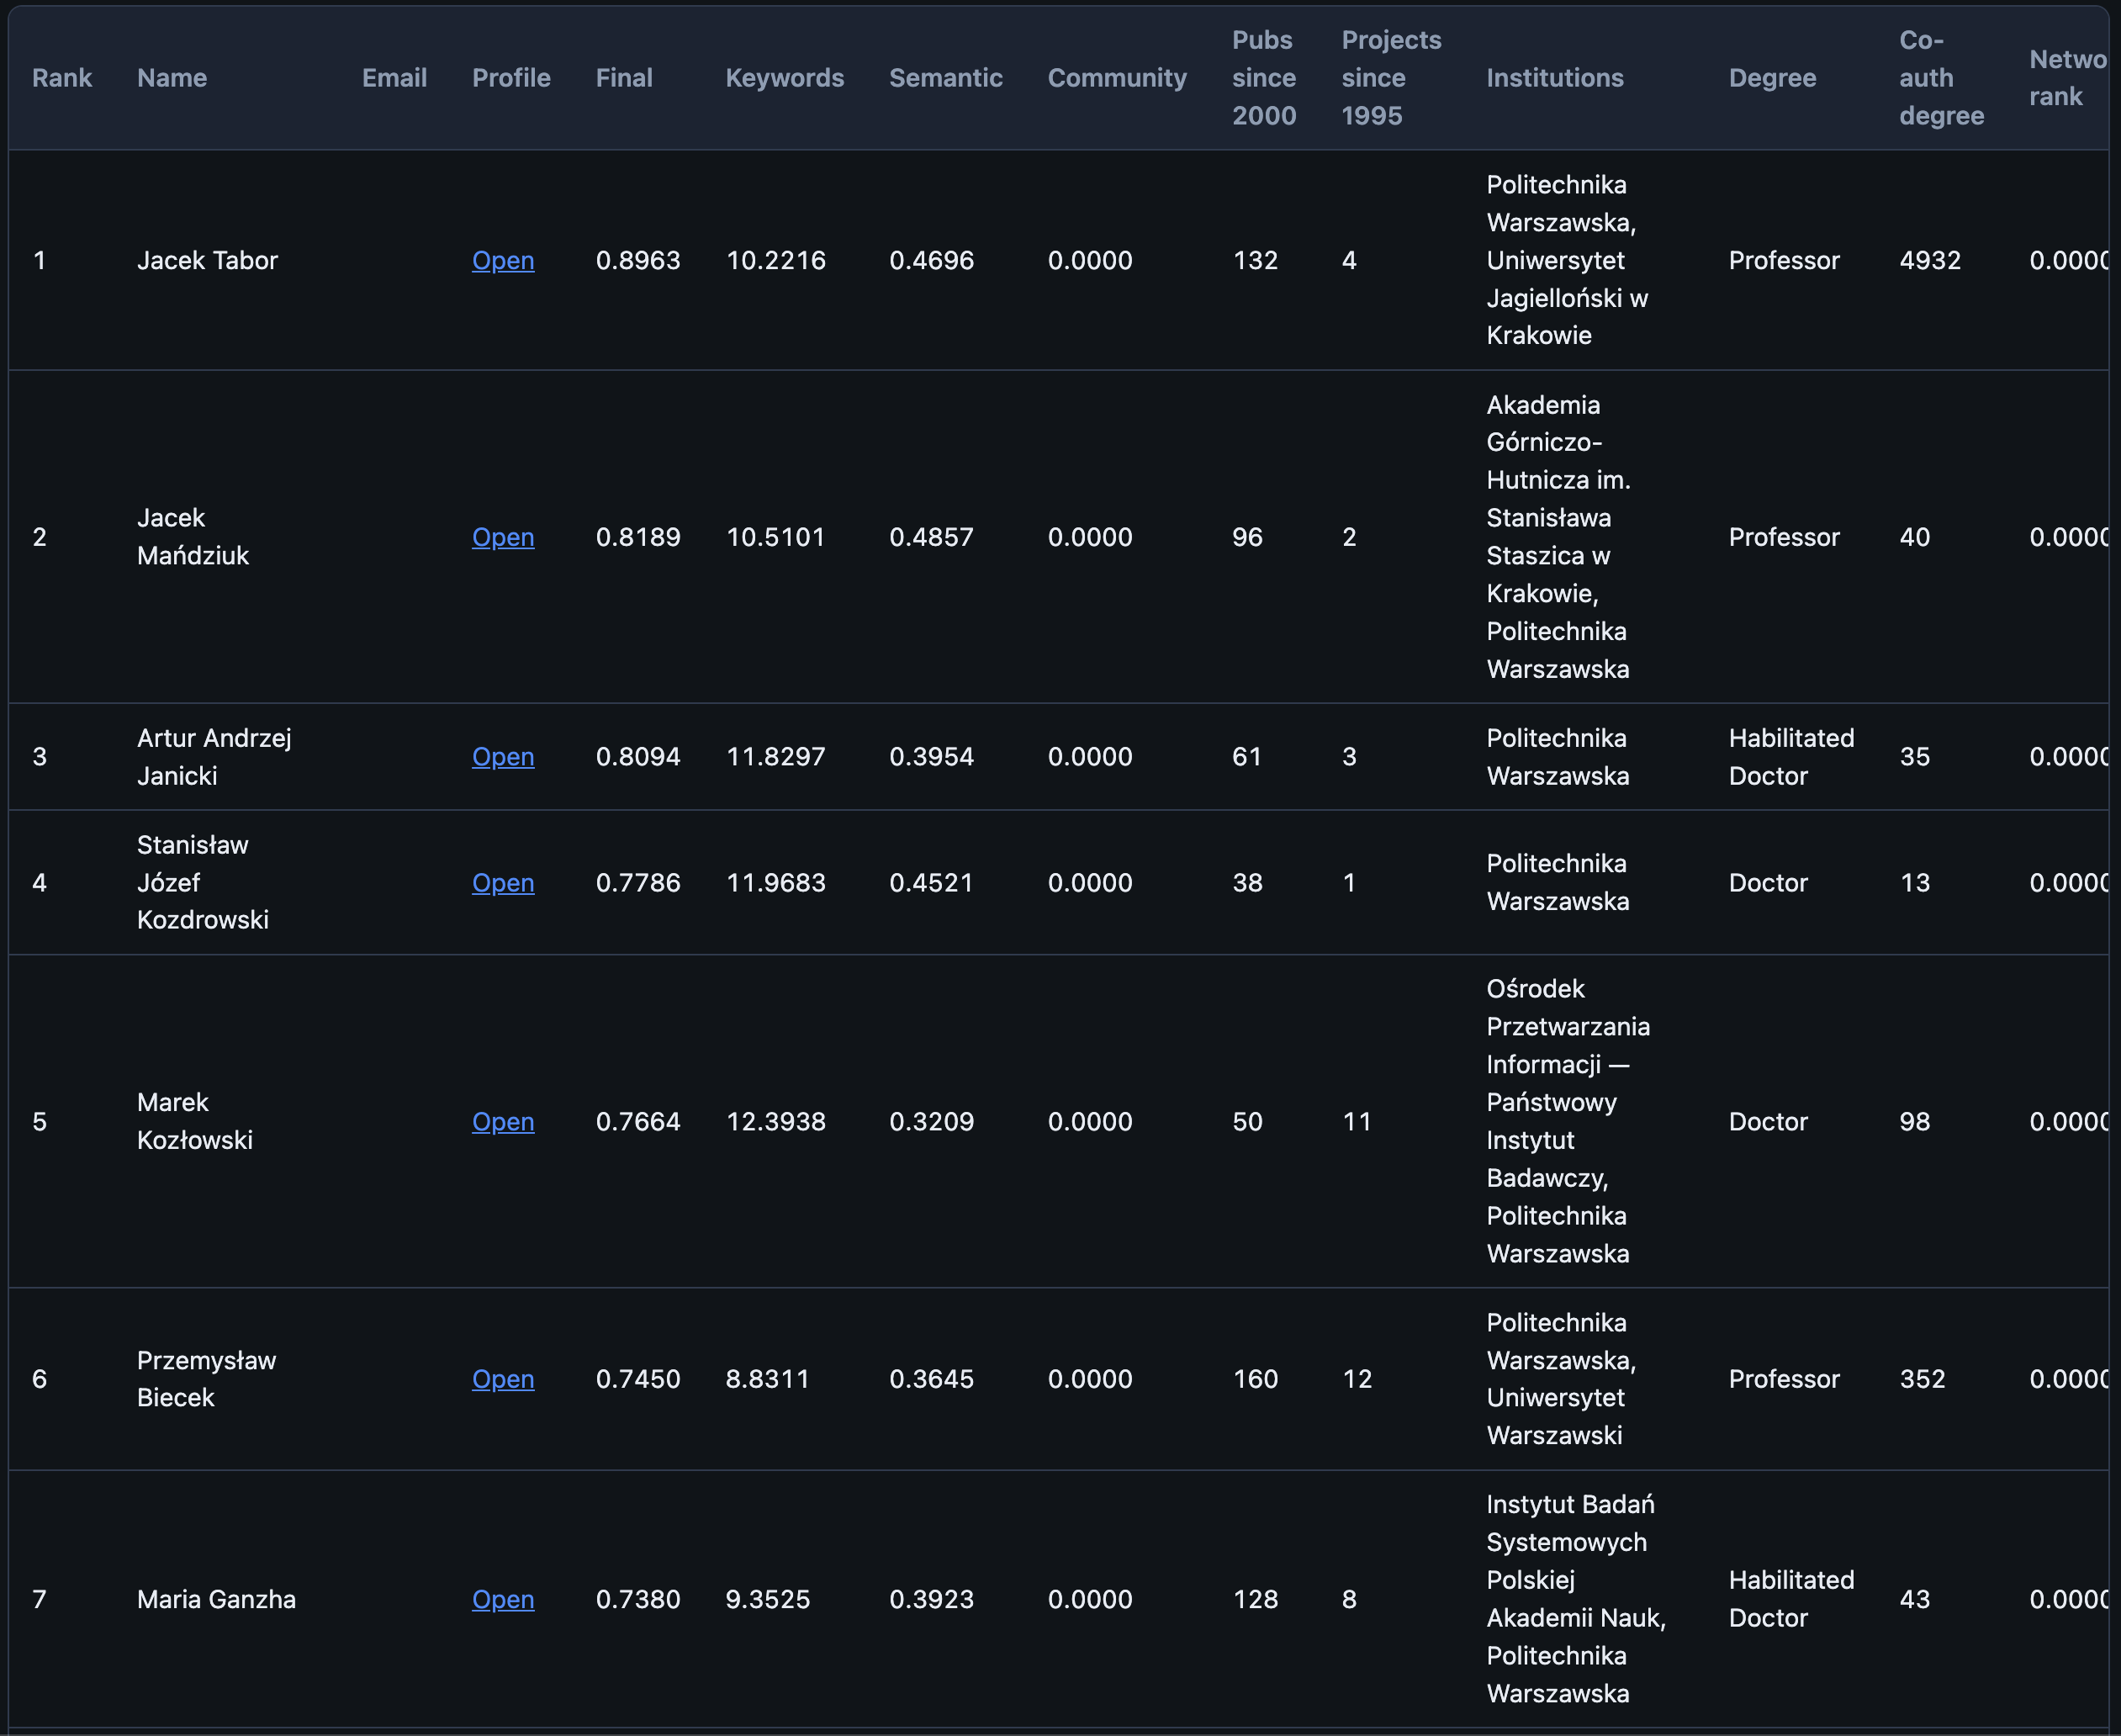
\includegraphics[width=\linewidth]{app_example_ranking_1.png}
        \vspace{0.15cm}
        {\scriptsize Results: Final, Keywords, Semantic, Community, network columns.}
        \vspace{0.2cm}
        \begin{itemize}
            \item FastAPI + static UI; CSV export (UTF-8 BOM for Excel).
            \item \textbf{pytest} suite: fusion, API, filters, graph metrics --- \texttt{uv run pytest}.
        \end{itemize}
    \end{columns}
\end{frame}


\end{document}